% -*- root: Document.tex -*-

\chapter{\SS{} Prototype}
\label{chap:proto}

\SS{} is implemented in \textsc{Lua} (v5.3).
The implementation of the middleware itself requires careful engineering, especially with respect to the integration in the SGX enclaves (explained later).
However, a \SS{} use-case can be implemented in remarkably few lines of code.
For instance, the implementation of the map/filter/reduce accounts for only $120$ lines of code (without counting the dependencies).
The framework partially extends \rxl~\cite{github:rxlua}, a library for reactive programming in \textsc{Lua}.
\rxl provides to the developer the required API to design a data stream processing pipeline following a dataflow programming pattern~\cite{uustalu_essence_2005}.

Listing~\ref{pipeline-example} provides an example of a \rxl program (and consequently a \SS{} program) to compute the average age of a population by chaining \texttt{:map}, \texttt{:filter}, and \texttt{:reduce} functions.\footnote{Note that in our evaluation the code executed by each worker is confined into its own \textsc{Lua} file.}
The \texttt{:subscribe} function performs the subscription of 3 functions to the data stream.
Following the \emph{observer} design pattern~\cite{szallies_using_1997}, these functions are observers, while the data stream is an observable.

\SS{} dynamically ships the business logic for each component into a dedicated Docker container and executes it.
The communication between the Docker containers (the router and the worker components) happens through \zmq (v4.1.2) and the corresponding \textsc{Lua} bindings~\cite{github:lzmq}.
Basically, \SS{} abstracts the underlying network and computing infrastructure from the developer, by relying on \zmq and Docker.

Under the SGX threat model where the system software is completely untrusted, system calls are not allowed inside secure enclaves.
As a consequence, porting a legacy application or runtime, such as the \textsc{Lua} interpreter, is challenging.
To achieve this task, we traced all system calls made by the interpreter to the standard C library and replaced them by alternative implementations that either mimic the real behavior or discard the call.
Our changes to the vanilla \textsc{Lua} source code consist of the addition of about $600$ lines of code, or $2.5\,\mathit{\%}$ of its total size.
By doing so, \textsc{Lua} programs operating on files, network sockets or any other input/output device do not execute as they normally do outside the enclaves.
This inherent SGX limitation also reinforces the system security guarantees offered to the application developers.
The \SS{} framework safely ships the data and code to enclaves.
Hence, the \textsc{Lua} scripts executed within the SGX enclave do not use (read/write) files or sockets.
Wrapper functions are nevertheless installed in the SGX-enabled \luavm to prevent any of such attempts.

An additional constraint imposed by the secure SGX enclaves is the impossibility of dynamically linking code.
The reason is that the assurance that a given code is running inside a SGX-enabled processor is made through the measurement of its content when the enclave is created.
More specifically, this measurement is the result of \texttt{EREPORT} instruction, an SGX-specific report that computes a cryptographically secure hash of code, data and a few data structures, which overall builds a snapshot of the state of the enclave (including threads, memory heap size, etc.) and the processor (security version numbers, keys, etc.).
Allowing more code to be linked dynamically at runtime would break the assurance given by the attestation mechanism on the integrity of the code being executed, allowing for example an attacker to load a malicious library inside the enclave.

In the case of \textsc{Lua}, a direct consequence is the impossibility of loading \textsc{Lua} extensions using the traditional dynamic linking technique.
Every extension has to be statically compiled and packed with the enclave code.
To ease the development of \SS applications, we statically compiled \emph{json}~\cite{rfc7159}, and \emph{csv}~\cite{rfc4180} parsers within our enclaved \textsc{Lua} interpreter.
With these libraries, the size of the VM and the complete runtime still remains reasonably small, approximately $220\,\mathit{KB}$ ($19\,\mathit{\%}$ larger than the original).

\begin{figure}[t!]
  \centering
  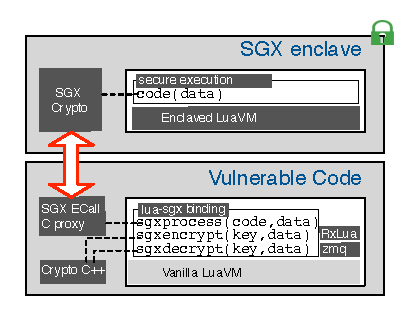
\includegraphics[width=.75\linewidth]{Figures/arch-sgxlua}
  \caption{Integration between \textsc{Lua} and Intel{\textregistered} SGX.}
  \label{fig:arch-luasgx}
\end{figure}

While this restricted \textsc{Lua} has been adapted to run inside SGX enclaves, we still had to provide a support for communications and the reactive streams framework itself.
To do so, we use an external vanilla \textsc{Lua} interpreter, with a couple adaptations that allowed the interaction with the SGX enclaves and the \luavm therein.
Figure~\ref{fig:arch-luasgx} shows the resulting architecture.
We extend the \textsc{Lua} interface with 3 functions: \texttt{sgxprocess}, \texttt{sgxencrypt}, and \texttt{sgxdecrypt}.
The first one forwards the encrypted code and data to be processed in the enclave, while the remaining two provide cryptographic functionalities.
In this work, we assume that attestation and key establishment was previously performed.
As a result, keys safely reside within the enclave.
We plan to release our implementation as open-source.

\newpage

\begin{minipage}{\linewidth}
\begin{lstlisting}[language=LUA,caption={Example of process pipeline with RxLua.},label=pipeline-example]
Rx.Observable.fromTable(people)
 :map(
   function(person)
     return person.age
   end
 )
 :filter(
   function(age)
     return age > 18
   end
 )
 :reduce(
   function(accumulator, age)
     accumulator[count] = (accumulator.count
       or 0) + 1
     accumulator[sum] = (accumulator.sum
       or 0) + age
     return accumulator
   end
 )
 :subscribe(
   function(datas)
     print("Adult people average:",
       datas.sum / datas.count)
   end,
   function(err)
     print(err)
   end,
   function()
     print("Process complete!")
   end
 )
\end{lstlisting}
\end{minipage}
